\section{OfbizCurrencyTransform}
This section provides an overview of the functional role of the \textcolor{blue}{OfbizCurrencyTransform} class and its methods. 
In this case we are considering a Freemarker Transform for content links.
As defined by the Apache Freemarker website\footnote{http://freemarker. org/}:

"Apache FreeMarker is a template engine: a Java library to generate text output (HTML web pages, e-mails, configuration files, source code, etc.) based on templates and changing data. Templates are written in the FreeMarker Template Language (FTL), which is a simple, specialized language (not a full-blown programming language like PHP). You meant to prepare the data to display in a real programming language, like issue database queries and do business calculations, and then the template displays that already prepared data. In the template you are focusing on how to present the data, and outside the template you are focusing on what data to present."

This class contains the declaration of a particular type of Freemarker, in particular its main function is to extract and transform the Java object received(Map of arguments), that in this case contain currency values and display them in an appropriate format. To do that the class implements the \textcolor{blue}{TemplateTransformModel}, that offer a common transform model for the FreeMarker, and specify it for the specific case of currency.

In order to accomplish this task, inside the class the are 4 methods:
\begin{itemize}
\item \textcolor{blue}{getArg}
\item \textcolor{blue}{getAmount}
\item \textcolor{blue}{getInteger}
\item \textcolor{blue}{getWriter}
\end{itemize}

The first three methods are very similar, in fact they receive the same input(a Map of arguments and a String that has the function of key) and return the argument corresponding to the key, if it exists. The only main difference between these three methods is the type of argument returned.
The fourth method \textcolor{blue}{getWriter} use the three methods defined before to get some specific values from the Map of arguments received in input and extract the following values: \textcolor{blue}{amount}, \textcolor{blue}{isoCode} and \textcolor{blue}{locale}.
Then the methods handles the rounding of the currency and finally it write on a buffer the data extracted in an appropriate format. This passage in made by overriding the methods \textcolor{blue}{write}, \textcolor{blue}{flush} and \textcolor{blue}{close} of the \textcolor{blue}{TemplateTransformModel}.

We include here the figure of the behaviour of the Apache Freemarker:
\begin{figure}[b]
\centering
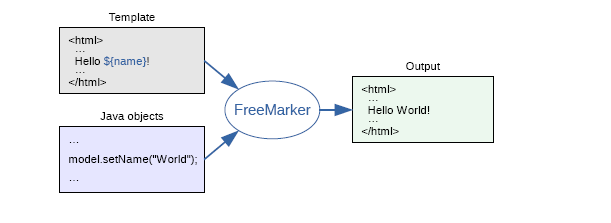
\includegraphics{functional_role/Images/freemarker.png}
\caption{Apache FreeMarker}\label{fig:1}
\end{figure}


